\documentclass[aspectratio=169]{beamer}

\mode<presentation>
{
  \usetheme{default}
  \usecolortheme{default}
  \usefonttheme{default}
  \setbeamertemplate{navigation symbols}{}
  \setbeamertemplate{caption}[numbered]
  \setbeamertemplate{footline}[frame number]  % or "page number"
  \setbeamercolor{frametitle}{fg=white}
  \setbeamercolor{footline}{fg=black}
} 

\usepackage[english]{babel}
\usepackage[utf8x]{inputenc}
\usepackage{tikz}
\usepackage{courier}
\usepackage{array}
\usepackage{bold-extra}
\usepackage{minted}
\usepackage[thicklines]{cancel}

\xdefinecolor{dianablue}{rgb}{0.18,0.24,0.31}
\xdefinecolor{darkblue}{rgb}{0.1,0.1,0.7}
\xdefinecolor{darkgreen}{rgb}{0,0.5,0}
\xdefinecolor{darkgrey}{rgb}{0.35,0.35,0.35}
\xdefinecolor{darkorange}{rgb}{0.8,0.5,0}
\xdefinecolor{darkred}{rgb}{0.7,0,0}
\definecolor{darkgreen}{rgb}{0,0.6,0}
\definecolor{mauve}{rgb}{0.58,0,0.82}

\title[2017-10-11-rootioworkshop-petabyte-file]{How to make a petabyte ROOT file: \\ proposal for managing data with columnar granularity}
\author{Jim Pivarski}
\institute{Princeton University -- DIANA}
\date{October 11, 2017}

\usetikzlibrary{shapes.callouts}

\begin{document}

\logo{\pgfputat{\pgfxy(0.11, 7.4)}{\pgfbox[right,base]{\tikz{\filldraw[fill=dianablue, draw=none] (0 cm, 0 cm) rectangle (50 cm, 1 cm);}
\includegraphics[height=1 cm]{diana-hep-logo.png}}}}

\begin{frame}
  \titlepage
\end{frame}

% Uncomment these lines for an automatically generated outline.
%\begin{frame}{Outline}
%  \tableofcontents
%\end{frame}

%%%%%%%%%%%%%%%%%%%%%%%%%%%%%%%%%%%%%%%%%%%%%%%%%%%%%%%

%%%% START

\begin{frame}[fragile]{Motivation: start by stating the obvious}
\vspace{0.15 cm}
ROOT's selective reading is very important for analysis.

\vspace{0.25 cm}
Datasets have about a thousand branches\footnote{3116 ATLAS MC, 1717 ATLAS data, 2151 CMS MiniAOD, 675+ CMS NanoAOD, 560 LHCb}, so if you want to plot a quantity from a terabyte dataset with {\tt TTree::Draw}, you only have to read a few gigabytes from disk.

\begin{uncoverenv}<2->
\vspace{1 cm}
Same for reading over a network (XRootD).
\begin{verbatim}
auto file = TFile::Open("root://very.far.away/mydata.root");
\end{verbatim}
\end{uncoverenv}

\vspace{0.1 cm}
\begin{uncoverenv}<3->
\begin{center}
\LARGE \underline{This is GREAT.}
\end{center}
\end{uncoverenv}
\end{frame}

\begin{frame}{Conversation with CS colleague}
\vspace{0.5 cm}
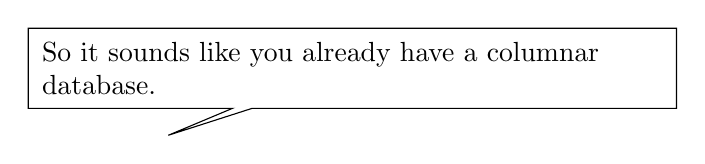
\begin{tikzpicture}[>=latex]
\node[rectangle callout, draw, inner sep=5 pt, callout relative pointer={(200:1 cm)}, text width=0.65\linewidth] {So it sounds like you already have a columnar database.};
\end{tikzpicture}

\vspace{0.25 cm}
\begin{uncoverenv}<2->
\hfill 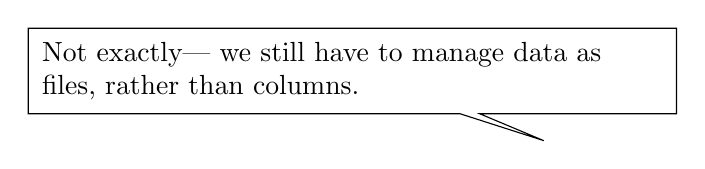
\begin{tikzpicture}[>=latex]
\node[rectangle callout, draw, inner sep=5 pt, callout relative pointer={(-200:-1 cm)}, text width=0.65\linewidth] {Not exactly--- we still have to manage data as files, rather than columns.};
\end{tikzpicture}
\end{uncoverenv}

\vspace{0.25 cm}
\begin{uncoverenv}<3->
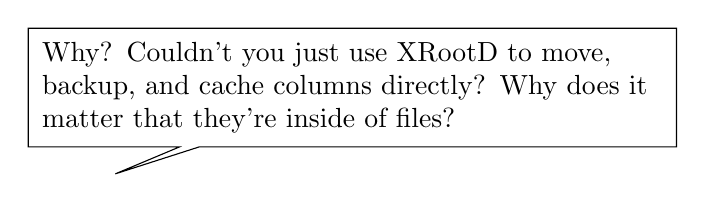
\begin{tikzpicture}[>=latex]
\node[rectangle callout, draw, inner sep=5 pt, callout relative pointer={(200:1 cm)}, text width=0.65\linewidth] {Why? Couldn't you just use XRootD to move, backup, and cache columns directly? Why does it matter that they're inside of files?};
\end{tikzpicture}
\end{uncoverenv}

\vspace{0.25 cm}
\begin{uncoverenv}<4->
\hfill 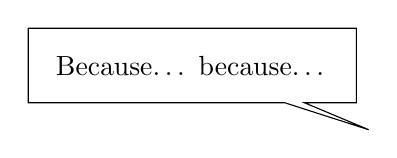
\begin{tikzpicture}[>=latex]
\node[rectangle callout, draw, inner sep=10 pt, callout relative pointer={(-200:-1 cm)}] {Because\ldots\ because\ldots};
\end{tikzpicture}
\end{uncoverenv}
\end{frame}

\begin{frame}{Proof that it matters: CMS NanoAOD}
\vspace{0.75 cm}
\textcolor{darkblue}{\underline{Stated goal:}} {to serve 30--50\% of CMS analyses with a single \underline{selection of columns.}}

\vspace{0.5 cm}
Painful decisions need to be made to keep disk size down to 1--2~kB/event, to make data access easier for 50\% of analyses while completely excluding others.

\vspace{0.5 cm}
\begin{columns}
\column{0.55\linewidth}
\begin{center}
\uncover<2->{If we could really manage data at the columnar level, we could just put the most frequently used 1--2~kB/event in warm storage and the other 40~kB/event in colder storage.}
\end{center}

\column{0.4\linewidth}
\begin{center}
\uncover<3->{Instead, we'll probably put the whole small copy (NanoAOD) in warm storage and the whole large copy (MiniAOD) in colder storage.}
\end{center}
\end{columns}

\vspace{0.25 cm}
\begin{center}
\uncover<4->{There is a steep popularity distribution across {\it columns,} \\ cut abruptly and artificially by what's in a {\it file}.}
\end{center}
\end{frame}

\begin{frame}{}
\vspace{0.5 cm}
\begin{center}
\large Except for the simplest TTree structures, we can't pull individual branches \\ out of a file and manage them on their own, because only ROOT knows how \\ to interpret a branch's relationship with other branches.

\vspace{1 cm}
\uncover<2->{BulkIO can extract branch data as arrays, bypassing the reconstruction into events, but only for certain branch types (``non-destructively serialized'').}
\end{center}
\end{frame}

\begin{frame}[fragile]{What would it look like if we could?}
\begin{minted}{sql}
CREATE TABLE derived_data AS
    SELECT pt, eta, phi, deltaphi**2 + deltaeta**2 AS deltaR
    FROM original_data WHERE deltaR < 0.2;
\end{minted}

creates a new {\tt derived\_data} table from {\tt original\_data}, but {\it links}, rather than {\it copying}, {\tt pt}, {\tt eta}, and {\tt phi}.\footnote{Implementation dependent, but common. ``{\tt WHERE}'' selection may be implemented with a stencil.}

\vspace{0.25 cm}
\uncover<2->{If {\tt original\_data} is deleted, the database would not delete {\tt pt}, {\tt eta}, and {\tt phi}, as they're in use by {\tt derived\_data}.}

\vspace{0.5 cm}
\uncover<3->{\textcolor{darkblue}{\underline{For data management,}} this is a highly fluid system, as columns are a more granular unit for caching and replication.}

\vspace{0.25 cm}
\uncover<4->{\textcolor{darkblue}{\underline{For users,}} there is much less cost to creating derived datasets--- many versions of corrections and cuts.}
\end{frame}

\begin{frame}{}
\vspace{1 cm}
\begin{center}
\Large \textcolor{darkblue}{\underline{Idea~\#1}.} Cast data from ROOT files into a well-known \\ standard for columnar, hierarchical data; manage those \\ columns individually in an object store like Ceph.
\end{center}

\begin{enumerate}
\item<2-> \textcolor{darkblue}{Apache Arrow} is one such standard. It's similar to ROOT's splitting format but continues splitting to all levels of depth.
\item<3-> \textcolor{darkblue}{PLUR or PLURP} is my subset of the above with looser rules about how data may be referenced. Acronym for the minimum data model needed for physics: {\bf Primitives}, {\bf Lists}, {\bf Unions}, {\bf Records}, and maybe {\bf Pointers} (beyond Arrow).
\end{enumerate}

\begin{center}
\uncover<4->{\Large (the ``database-like'' approach)}
\end{center}
\end{frame}

\begin{frame}{}
\vspace{1 cm}
\begin{center}
\Large \textcolor{darkblue}{\underline{Idea~\#2} (this talk).} Keep ROOT data as they are, but put \\ individual {\it baskets} in the object store. TFile/TTree subclasses fetch data from the object store instead of seeking to file positions.
\end{center}

\begin{enumerate}
\item<2-> Presents the same TFile/TTree interface to users; old scripts still work.
\item<3-> But data replication, storage class, and caching are handled by the object store with columnar granularity.
\item<4-> Branches are shared transparently across derived datasets: all trees are friends.
\item<5-> The logic of sharing, reference counting branches, managing datasets, etc.\ must all be implemented in ROOT; only ROOT understands how to combine branches.
\end{enumerate}

\begin{center}
\uncover<6->{\Large (the ``ROOT eats the world'' approach)}
\end{center}
\end{frame}

\begin{frame}{How it could be done}
\vspace{0.3 cm}
\begin{itemize}
\item<1-> Subclass of TFile configures itself by contacting a ``controlling'' database (document store like MongoDB might be best).
\item<2-> Reference counts for objects referenced by TKeys (including TBaskets and user objects like histograms) are maintained by the controlling database.
\item<3-> Bulk data, the contents of TKeys, are in a ``warehouse'' database (object store--- \mbox{\it might} be the same database). Optimal basket size may be big, like megabytes.
\item<4-> REST APIs for flexibility. No database clients as new ROOT dependencies. TBaskets are fetched by HTTP GET.
\item<5-> New TTrees derived from old TTrees\ldots
\begin{itemize}
\item<6-> share common TBranch data by default;
\item<7-> ``soft skim'' by stencil (event list/event bitmap), ``hard skim'' only if re-basketization is needed to compactify results (keeping fewer than $\sim$10\% of original);
\item<8-> save all provenance and use git-like history to determine if two branches are related/may be combined (for a join by index, rather than mutual column).
\end{itemize}
\item<9-> No user-facing partition boundaries: huge dataset appears as one TTree.
\item<10-> Users work in shared TFile: home TDirectories; permissions managed by database.
\end{itemize}
\end{frame}

\begin{frame}{Modes of use}
\vspace{0.5 cm}
\begin{block}{Direct connection}
Users launch ROOT, open a {\tt TFile("rootdb://data.cern/cms")}, and extract objects for plotting/analysis: {\tt Get("home/username/myhist").Draw()}.
\end{block}

\vspace{0.5 cm}
\begin{uncoverenv}<2->
\begin{block}{Job submission}
Users pass macros, {\tt TTree::Draw} requests, or {\tt TDataFrame} tasks to a service that parallelizes them and puts results in the user's home TDirectory.

\begin{itemize}
\item<3-> compute nodes use this same interface to communicate with storage;
\item<4-> but a scheduler attempts to maximize shared cache locality on the compute nodes.
\end{itemize}
\end{block}
\end{uncoverenv}

\vspace{0.25 cm}
\begin{center}
\large \uncover<5->{This is the ``query server'' idea I've been exploring form some time now, \\ except that all of the interface is ROOT.}
\end{center}
\end{frame}

\begin{frame}{}
\vspace{1.25 cm}
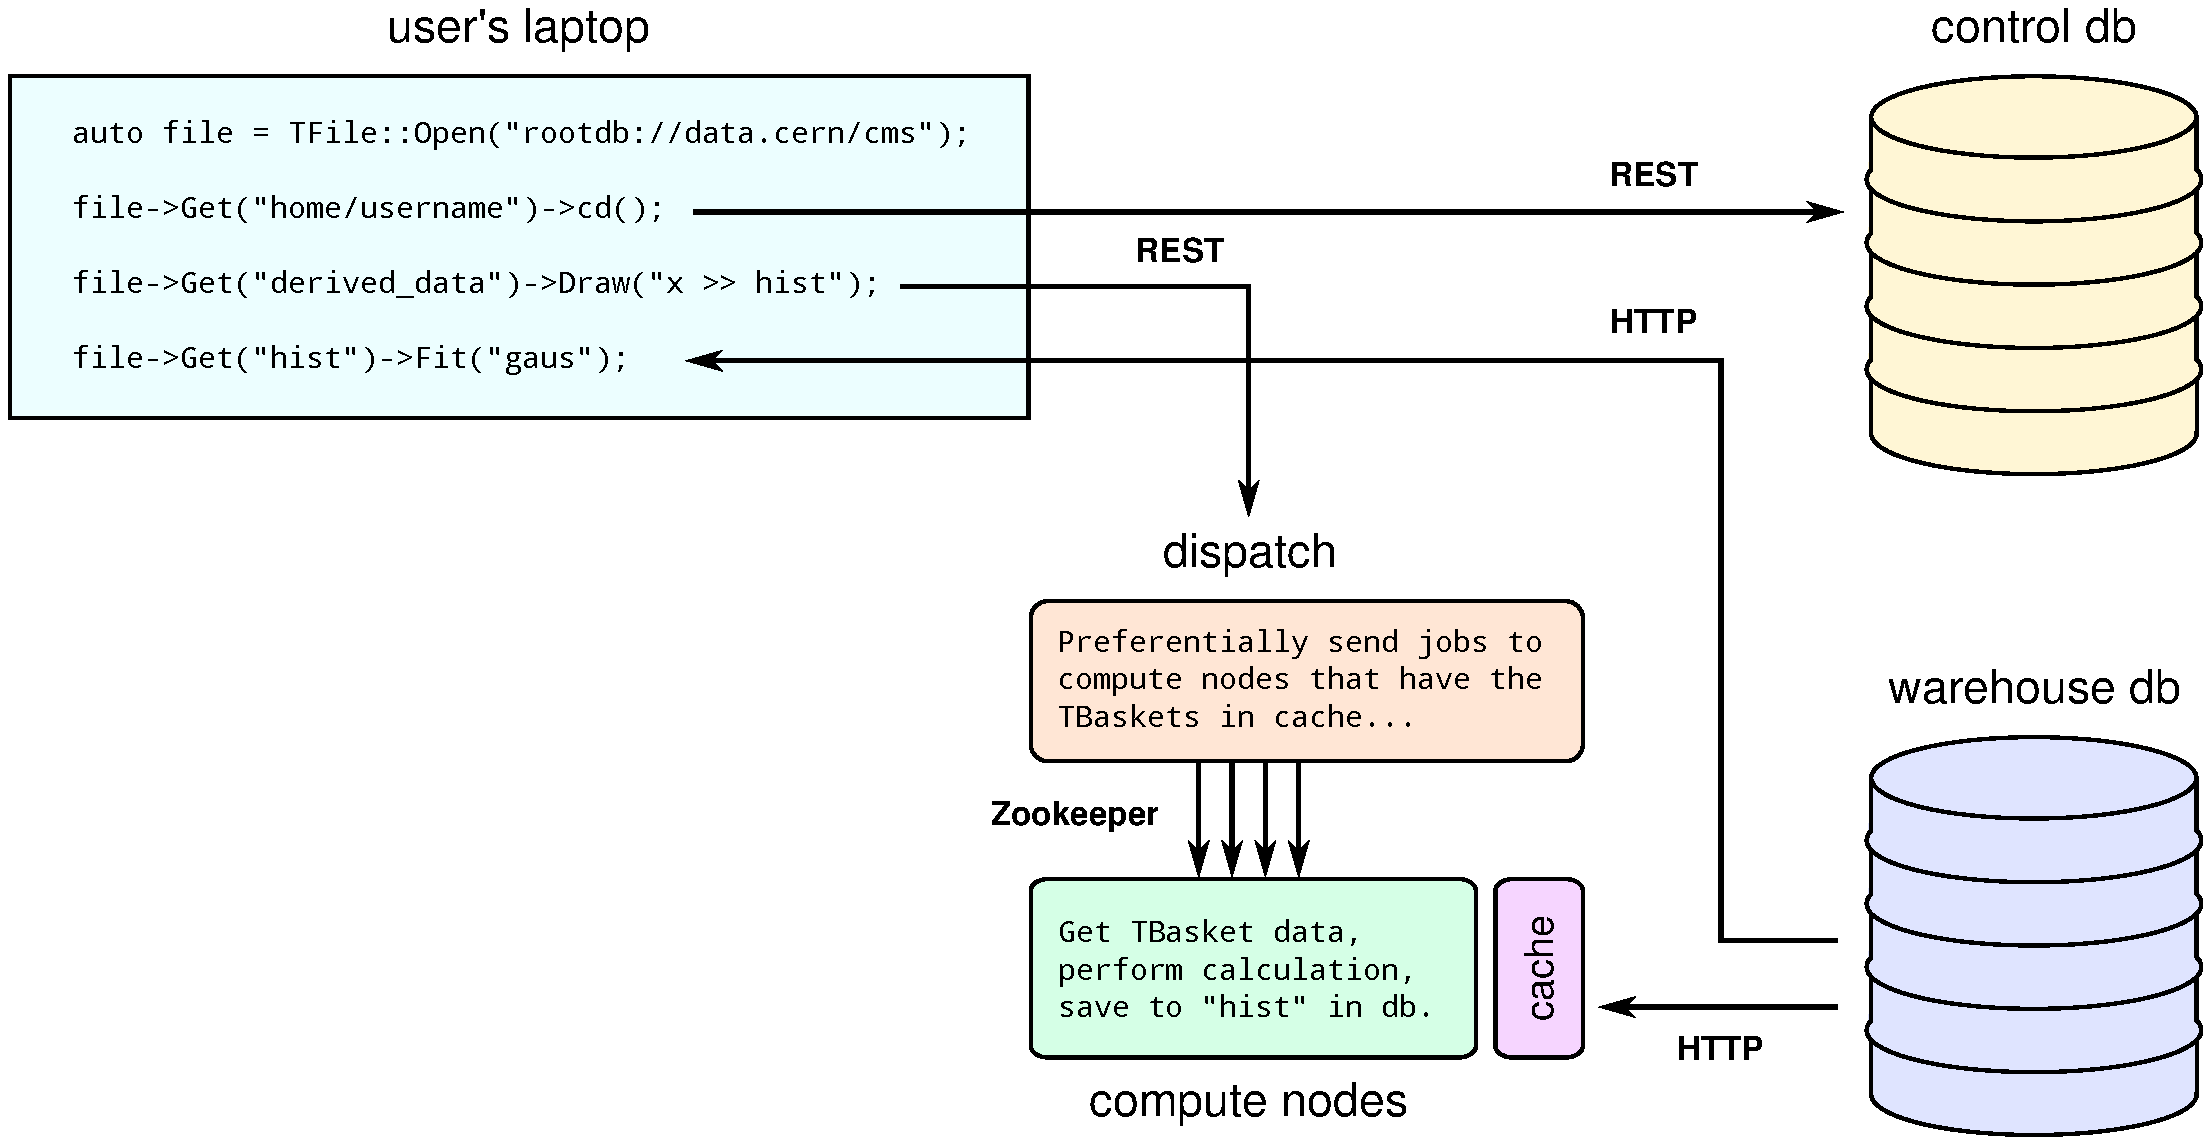
\includegraphics[width=\linewidth]{root-query-system.pdf}
\end{frame}

\begin{frame}{Questions for you}
\vspace{0.5 cm}
\begin{description}\setlength{\itemsep}{0.5 cm}
\item[Question:] How would you feel if I developed this kind of service {\it within} ROOT (\textcolor{darkblue}{idea~\#2}), rather than outside of ROOT (\textcolor{darkblue}{idea~\#1})?

\vspace{0.25 cm}
\uncover<2->{I'd want to sketch it out in Python (uproot) to figure out the architecture before committing to the ROOT codebase: $\sim$year timescale.}

\item[Question:]<3-> Deeply nested columnar splitting, zero-copy structure manipulations, and many database indexing techniques are not possible with today's ROOT serialization.

\vspace{0.25 cm}
\uncover<4->{Are you interested in forward-incompatible changes to ROOT serialization that would make these things possible? I could propose them as a ROOT 7 serialization format.}

\vspace{0.25 cm}
\uncover<5->{(Subject of another talk.)}
\end{description}
\end{frame}
\end{document}
